\section{Exploratory Runs}\label{sec:results-exploratory}

This study began with runs made on 2026-10-06, before the protocol of Section~\ref{sec:method} existed. They are why
the protocol looks the way it does, and they are kept here for that reason, apart from the controlled results and
never mixed into their tables.

\noindent\fcolorbox{orange}{white}{\parbox{0.97\linewidth}{\small\textbf{\expl.} Everything in this section comes from
one run per configuration on a single pod, with all requests of a load level sent at once, usable bars chosen after
seeing the data, and no quality evaluation. The files are imported verbatim with hashes
(\datafile{data/exploratory/MANIFEST.tsv}), and the statistics below are recomputed from them by
\datafile{src/hostoffload/analysis/exploratory.py}.}}

\paragraph{What the first sweep showed.}
The sweep ran closed loops from $N=1$ to 64 users on the \texttt{\dv{expl.plan_identified.sweep}} plan
(Tables~\ref{tab:expl-sweep-A} and~\ref{tab:expl-sweep-B}, Figure~\ref{fig:expl-sweep}). With unique 4K-token code
prompts (scenario A), one request decoded at a median of \dv{expl.A.N1.decode_p50_tok_s} tokens/s and waited
\dv{expl.A.N1.ttft_p50_s}\,s for its first token. At eight users the median rate per request was
\dv{expl.A.N8.decode_p50_tok_s} tokens/s and at 64 it was \dv{expl.A.N64.decode_p50_tok_s}. The total output grew only
\dv{expl.A.agg_ratio_8_1}-fold from one user to eight and \dv{expl.A.agg_ratio_64_1}-fold to 64
(\dv{expl.A.N64.aggregate_out_tok_s} tokens/s). With a cached 16K-token prefix (scenario B) the total reached
\dv{expl.B.N64.aggregate_out_tok_s} tokens/s at 64 users and the median TTFT stayed at \dv{expl.B.N64.ttft_p50_s}\,s.
There were \dv{expl.A.errors_total} errors in \dv{expl.A.requests_total} requests in A and \dv{expl.B.errors_total} in
\dv{expl.B.requests_total} in B. This is the shape the controlled sweep later confirmed: concurrency buys total
throughput with each user's speed.

% Generated by hostoffload.analysis.pipeline. Do not edit.
\begin{table}[t]
\centering
\small
\begin{fittable}{tab:expl-sweep-A}
\begin{tabular}{rrrrrrrrrr}
\toprule
$N$ & $n$ & TTFT p50 & TTFT p95 & p95 later & decode p50 [CI] & p5 & aggr. & accept & USD/M out \\
\midrule
1 & 8 & 0.96 & 1.02 & 1.02 & 116.2 [113.0, 125.0] & 111.2 & 82.1 & 3.28 & 14.15 \\
2 & 8 & 0.99 & 1.80 & 1.80 & 70.9 [63.0, 94.7] & 54.0 & 112.2 & 3.39 & 10.35 \\
4 & 8 & 1.48 & 3.11 & 2.03 & 40.1 [33.8, 60.2] & 30.0 & 126.0 & 3.29 & 9.22 \\
8 & 16 & 2.04 & 4.99 & 2.55 & 23.1 [21.5, 26.3] & 16.7 & 152.1 & 3.37 & 7.63 \\
16 & 32 & 3.39 & 9.20 & 3.42 & 13.8 [13.3, 15.2] & 9.4 & 176.0 & 3.38 & 6.60 \\
32 & 64 & 5.05 & 18.47 & 5.82 & 8.2 [7.7, 9.1] & 5.8 & 209.3 & 3.37 & 5.55 \\
64 & 128 & 8.34 & 33.48 & 8.70 & 4.6 [4.3, 4.8] & 3.4 & 234.1 & 3.34 & 4.96 \\
\bottomrule
\end{tabular}
\end{fittable}
\par\smallskip\parbox{0.95\linewidth}{\footnotesize\raggedright Source: \texttt{data/exploratory/inferencekey-deepseek@546071a/vllm-exl3/pro6000-concurrency/results/scenario\_A.json}. ``p95 later'': TTFT p95 of requests sent after the first wave. Price: \texttt{experiments/pricing.yaml}.}
\caption{\textbf{EXPLORATORY} (single run, burst arrivals, not controlled). Scenario A: independent requests, a different 4K-token code prompt each (0 prefix-cache hits); 256 output tokens, closed loop, 2x RTX PRO 6000, DSpark $k=5$. TTFT and decode percentiles are nearest rank on $n$ requests (p95 is close to the maximum for $n<20$). Bracket: 95\% request-level bootstrap interval of the median, which ignores run-to-run variance. Cost: output-only attribution at the measured aggregate rate.}
\label{tab:expl-sweep-A}
\end{table}

% Generated by hostoffload.analysis.pipeline. Do not edit.
\begin{table}[t]
\centering
\small
\begin{fittable}{tab:expl-sweep-B}
\begin{tabular}{rrrrrrrrrr}
\toprule
$N$ & $n$ & TTFT p50 & TTFT p95 & p95 later & decode p50 [CI] & p5 & aggr. & accept & USD/M out \\
\midrule
1 & 8 & 0.41 & 0.49 & 0.42 & 136.4 [127.1, 149.6] & 121.8 & 113.0 & 3.87 & 10.28 \\
2 & 8 & 0.43 & 0.81 & 0.44 & 95.5 [84.5, 101.6] & 72.0 & 149.5 & 3.92 & 7.77 \\
4 & 8 & 0.49 & 0.94 & 0.79 & 61.7 [53.2, 72.4] & 51.2 & 208.2 & 3.90 & 5.58 \\
8 & 16 & 1.01 & 1.31 & 1.31 & 31.5 [29.7, 37.3] & 23.8 & 223.7 & 3.90 & 5.19 \\
16 & 32 & 1.44 & 1.81 & 1.81 & 18.8 [18.0, 20.8] & 15.0 & 264.8 & 3.95 & 4.38 \\
32 & 64 & 2.09 & 10.32 & 2.09 & 11.1 [10.7, 11.6] & 9.0 & 270.1 & 3.95 & 4.30 \\
64 & 128 & 2.23 & 4.39 & 2.45 & 7.1 [6.9, 7.3] & 6.0 & 398.2 & 4.03 & 2.92 \\
\bottomrule
\end{tabular}
\end{fittable}
\par\smallskip\parbox{0.95\linewidth}{\footnotesize\raggedright Source: \texttt{data/exploratory/inferencekey-deepseek@546071a/vllm-exl3/pro6000-concurrency/results/scenario\_B.json}. ``p95 later'': TTFT p95 of requests sent after the first wave. Price: \texttt{experiments/pricing.yaml}.}
\caption{\textbf{EXPLORATORY} (single run, burst arrivals, not controlled). Scenario B: 16K-token shared code prefix (cached) plus a short question; 256 output tokens, closed loop, 2x RTX PRO 6000, DSpark $k=5$. TTFT and decode percentiles are nearest rank on $n$ requests (p95 is close to the maximum for $n<20$). Bracket: 95\% request-level bootstrap interval of the median, which ignores run-to-run variance. Cost: output-only attribution at the measured aggregate rate.}
\label{tab:expl-sweep-B}
\end{table}


\paragraph{Three lessons that shaped the protocol.}
The first is about arrivals. Sending every request of a level at the same instant inflates the tail. In A at 64 users
the TTFT p95 was \dv{expl.A.N64.ttft_p95_s}\,s over all requests and \dv{expl.A.N64.ttft_p95_after_first_wave_s}\,s
over the requests sent after the first wave (Figure~\ref{fig:expl-ttft}), so the controlled protocol staggers starts,
which our runs did, and adds Poisson arrivals, which were designed but not run. The second is about content. DSpark
accepted on average \dv{expl.A.N8.spec_mean_accept_len} tokens per step in A and \dv{expl.B.N8.spec_mean_accept_len}
in B at eight users, and in the first run 480-token prose answers (an essay and two explanations) decoded at
\dv{expl.first.decode_480_0.decode_tok_s} to \dv{expl.first.decode_480_1.decode_tok_s} tokens/s for one stream,
against \dv{expl.A.N1.decode_p50_tok_s} for code reviews. Speed depends on what the model writes, which is why the
protocol separates code from prose and has an experiment with speculation off (E7, designed but not run, so every
controlled run used code prompts with DSpark on). The third is about attribution. These runs cannot say what the
offload costs: there is no run without it, because it does not fit, no run at another host share and no reference with
everything in GPU memory. The slowdown with more users may come from reads of host experts, from the growth of the
batch that speculation verifies, from interference by new prompts, or from decode steps larger than the biggest CUDA
graph running without one. The ablations designed to separate these (E4 to E7) did not run, so the controlled results
do not separate them either.

\begin{figure}[t]
\centering
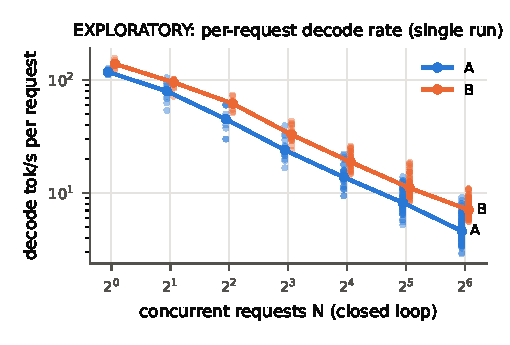
\includegraphics[width=0.49\linewidth]{figures/generated/exploratory_decode_per_request.pdf}\hfill
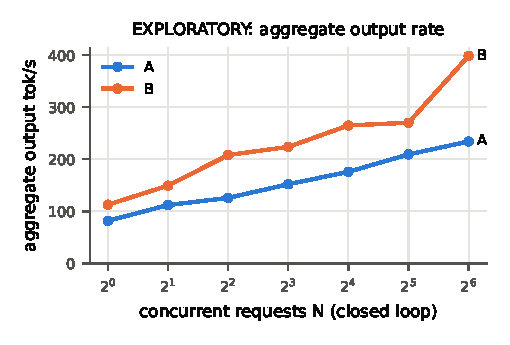
\includegraphics[width=0.49\linewidth]{figures/generated/exploratory_aggregate.pdf}
\caption{\expl{} (single run). Left: per-request decode rate (dots: requests, lines: medians) against concurrency.
Right: aggregate output rate. Sources: \texttt{scenario\_A.json} and \texttt{scenario\_B.json} in
\datafile{data/exploratory/inferencekey-deepseek@546071a/vllm-exl3/pro6000-concurrency/results/}.}
\label{fig:expl-sweep}
\end{figure}

\begin{figure}[t]
\centering
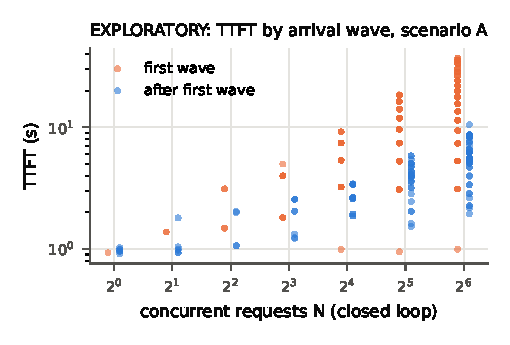
\includegraphics[width=0.49\linewidth]{figures/generated/exploratory_ttft_waves_A.pdf}\hfill
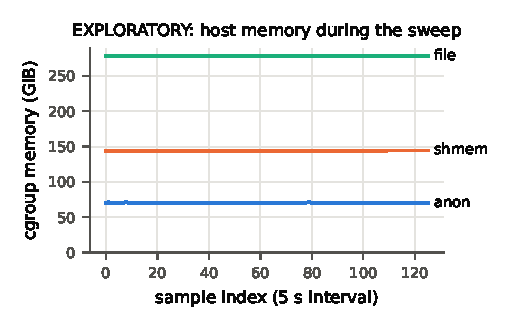
\includegraphics[width=0.49\linewidth]{figures/generated/exploratory_memory_timeline.pdf}
\caption{\expl{} (single run). Left: TTFT of first-wave requests (all sent at the start of a level) and of later
requests, scenario A. Right: host memory of the pod's cgroup during the sweep, 5\,s samples
(\texttt{mem\_samples.csv} in the folder of Figure~\ref{fig:expl-sweep}).}
\label{fig:expl-ttft}
\end{figure}

\paragraph{Memory stood still.}
The server reported \dv{expl.model_loading_gib}\,GiB of weights per GPU (loaded in \dv{expl.model_loading_s}\,s),
\dv{expl.cuda_graph_gib}\,GiB of CUDA graphs and a KV pool of \dv{expl.kv_tokens} tokens, enough for
\dv{expl.max_conc_x} requests at the full context limit. GPU memory stayed between \dv{expl.vram_min_peak_mib} and
\dv{expl.vram_peak_mib}\,MiB at every load level, because the pools are allocated in advance. Host memory did not move
with load either. Anonymous memory stayed between \dv{expl.ram_anon_min_gib} and \dv{expl.ram_anon_max_gib}\,GiB and
shared memory at \dv{expl.ram_shmem_gib}\,GiB, while the page cache filled the cgroup to
\dv{expl.ram_current_max_gib}\,GiB. The static split predicts \dv{static.gen30.host_gib}\,GiB of pinned file bytes for
this plan, more than the shared memory alone. These runs did not record how pinned buffers divide between anonymous
and shared mappings, and the controlled sampler dumps the largest mappings of every server process, but we have not
analyzed those dumps. Raising the context limit to 1M tokens raised the weight memory to
\dv{expl.1m.model_loading_gib}\,GiB and graphs to \dv{expl.1m.cuda_graph_gib}\,GiB per GPU and gave
\dv{expl.1m.kv_tokens} KV tokens from the same KV budget.

\paragraph{The first sign of prefix caching.}
In the first run a fresh code prompt of \dv{expl.first.ttft_16k.prompt_tokens} tokens took
\dv{expl.first.ttft_16k.ttft_s}\,s to its first token, and a second turn on the same prefix took
\dv{expl.first.ttft_16k_second_turn.ttft_s}\,s, with \dv{expl.first.ttft_16k_second_turn.cached} of
\dv{expl.first.ttft_16k_second_turn.prompt_tokens} prompt tokens served from the cache. That run's folder is named
\texttt{a100} after a sizing test, but it ran on the same 2x RTX PRO 6000 type
(\datafile{data/exploratory/inferencekey-deepseek@546071a/vllm-exl3/a100/results/agent30/bench.json}).

\paragraph{What the first sweep implied for cost.}
At the quoted pod price, with the whole hour charged to output tokens, the sweep implies
\dv{expl.A.N1.usd_per_m_out}\,USD per million output tokens for one user in A, \dv{expl.A.N8.usd_per_m_out} at eight
and \dv{expl.A.N64.usd_per_m_out} at 64, and \dv{expl.B.N1.usd_per_m_out}, \dv{expl.B.N8.usd_per_m_out} and
\dv{expl.B.N64.usd_per_m_out} in B. The cost per concurrent request falls as $1/N$, from \dv{expl.A.N1.usd_per_req_hour}
to \dv{expl.A.N64.usd_per_req_hour}\,USD per request-hour. Applying the pre-registered objectives (with TPOT p95
approximated by the inverse of the nearest-rank p5 decode rate, because that run did not store per-token times), the
interactive objective holds in A up to $N=\dv{expl.A.slo.interactive.N}$ at
\dv{expl.A.slo.interactive.usd_per_m_out}\,USD per million output tokens, the relaxed one up to
$N=\dv{expl.A.slo.relaxed.N}$ at \dv{expl.A.slo.relaxed.usd_per_m_out}\,USD, and the long-context one in B up to
$N=\dv{expl.B.slo.long_context.N}$ at \dv{expl.B.slo.long_context.usd_per_m_out}\,USD. With percentiles from 8 to 128
requests and burst arrivals, these numbers say where the frontier lies, not how precisely.
